\chapter{Load Analysis}
\label{ch:LoadAnalysis}
The wingbox shall be designed such that it can withstand the wing loads by providing sufficient stiffness. This Chapter will analyze the forces and moments acting on the wing and produce clear graphs of their variation along the structure. \autoref{sec:fd_modeling_approach_and_assumptions} states all simplifications and assumptions made for the wing model. The aerodynamic loading is then derived in \autoref{sec:fd_aerodynamic_loading_analysis} using XFLR5 simulations based on the wing geometry established in \textit{Wing Aerodynamic Design} \cite{Koppejan2024WingDesign}. Diagrams of the shear force, bending moment, and torque are constructed in \autoref{sec:fd_shear_moment_torque}. The most critical cases are presented and analyzed separately in \autoref{sec:fd_critical_cases}.

\section{Modeling Approach and Assumptions} \label{sec:fd_modeling_approach_and_assumptions}
%A list of assumptions made in the derivation of the axial force, shear force, bending moment, and torque diagrams.

This report aims to provide a rather \textit{preliminary} design of the wing. Therefore, several assumptions are made regarding the wing and loads to simplify the loading problem. This section describes the reasons for these steps, their validity, and the consequences they have on the results of the analysis.

\subsection*{Coordinate System}
% Note that the transformation to the tangential force component is not required for this assignment. (small angle of attack)
In the interest of avoiding confusion, it is important to define a suitable coordinate system. The XFLR5 simulations provide results in the \textit{body reference frame}, while the stiffness calculations are evaluated and graphically described for the \textit{aerodynamic reference frame} \cite{Timmer2024AE2111-IReader}.\\

\noindent The transformation of the lift and drag per unit span ($L'$ and $D'$, respectively) from the aerodynamic reference frame into a normal force $N'$ (see: \autoref{fig:forces_coordinate_transformation} \cite{Timmer2024AE2111-IReader}) in the body reference frame can be done according to \autoref{eq:forces_normal_transformation} \cite{Timmer2024AE2111-IReader}, \\

\begin{equation}    \label{eq:forces_normal_transformation}
    N'(y)=cos(\alpha)L'(y)+sin(\alpha)D'(y)
\end{equation}

\begin{figure}[H]
    \centering
    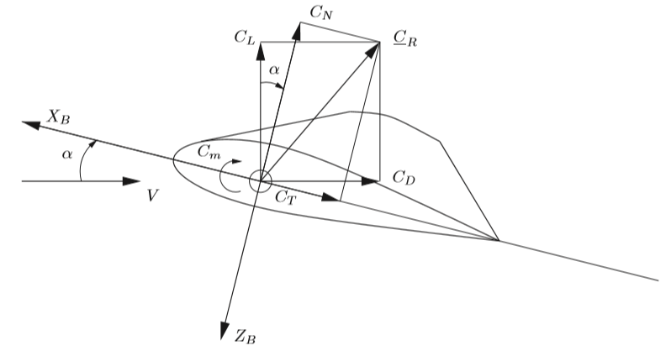
\includegraphics[width=0.5\linewidth]{figures/coordinates_converting_forces.png}
    \caption{Converting Aerodynamic Forces to Body Forces \cite{Timmer2024AE2111-IReader}}
    \label{fig:forces_coordinate_transformation}
\end{figure}


\noindent where $\alpha$ is the angle of attack. Note that for small values of $\alpha$, the normal force is approximately equal to the aerodynamic lift. Nonetheless, for some of the considered scenarios, the correction will have to be applied.\\

\noindent A simplified visualization of the wing loading, as well as the coordinate system used for the calculation of the shear, bending, and torsion, is showcased in \autoref{fig:candidate_coordinate_system}. For this analysis, A distributed force $w(x)$ will be considered, as well as the engine weight $P_E$, located at $x_E$.

\begin{figure}[H]
    \centering
    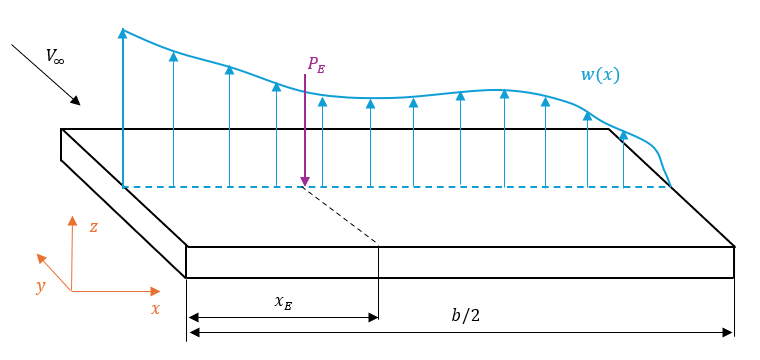
\includegraphics[width=0.75\linewidth]{figures/beam_loading_no_moment.png}
    \caption{Wing Loading Visualization}
    \label{fig:candidate_coordinate_system}
\end{figure}


\subsection*{Wing Sweep}
The planform design established in \textit{Wing Aerodynamic Design} \cite{Koppejan2024WingDesign} features a swept wing. Swept wings introduce complex load phenomena into the structure, which are outside of the scope of this course \cite{Timmer2024AE2111-IReader}. Therefore, a simpler shape will be considered for the construction of force and moment diagrams - an equivalent trapezoidal wing with a constant sweep angle (see: \autoref{fig:fd_assumptions_equivalent_unswept_wing}). The new model can be assumed to have the same values as the original wing, except for the sweep at the flexural axis, which is reduced from the original sweep angle $\Lambda$ to zero \cite{Timmer2024AE2111-IReader}.
\begin{figure}[h]
    \centering
    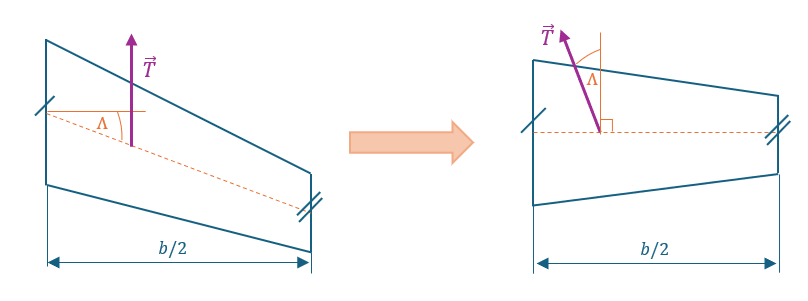
\includegraphics[width=0.85\linewidth]{figures/wing_sweep_effect.png}
    \caption{Equivalent unswept wing model}
    \label{fig:fd_assumptions_equivalent_unswept_wing}
\end{figure}

\noindent One consequence of this assumption is the changed direction of the thrust - as shown in \autoref{fig:fd_assumptions_equivalent_unswept_wing}, the orientation of the vector changes by an angle $\Lambda$. This happens because of the nature of the simplification - the whole planform is rotated to negate the effect of the sweep, and so is the thrust vector \cite{Timmer2024AE2111-IReader}.\\

\noindent The use of an equivalent trapezoidal wing is valid for modeling the variation of aerodynamic forces across the wing. However, it cannot be used in XFLR5 simulations, as the wing sweep affects the lift distribution, resulting in an overestimation of lift force towards the base of the wing, and an underestimation at the tips compared to the swept wing \cite{Timmer2024AE2111-IReader}.

\subsection*{In-Plane Forces and Moments}
The simplified loading case only considers shear forces in the vertical direction, i. e. perpendicular to the chord line. Therefore, the in-plane shear acting in the direction tangential to the chord line will be neglected. The same applies to bending moments - only those acting along the axis normal to the chord line are analyzed, and the in-plane bending of the wingbox will not be regarded.\\

\noindent Neglecting the in-plane loads will, indispensably, lead to an overestimation of the performance of the wingbox in terms of strength and stiffness. In-plane interferences may lead to structural fatigue and shear fractures in metals \cite{Yin2015AMaterials}. However, the contribution of these loads to the shear, bending, and torsion of the wingbox is negligible \cite{Timmer2024AE2111-IReader}, and hence, they are not considered in this part of the structural analysis.\\

\noindent Adding to these, the calculation of the shear force, bending moment, and torsion will only consider the contribution due to the wing loading and the engine weight. Thus the contribution due to the weight of the wing itself and the weight of the fuel will not considered. This assumption is deemed valid as it will lead to a conservative estimation of the forces.












%Note that formally speaking, point forces and couple moments can also be included in the distributed loading functions by use of Dirac-delta functions. However, for the sake of simplicity, point forces and couple moments will be treated separately from the distributed load.



\section{Aerodynamic Loading Analysis}  \label{sec:fd_aerodynamic_loading_analysis}
%Comment on the different reference frames for XFLR5 and force analysis [Fig. 9, p. 26 of the Reader].
The starting point of the load analysis is the computation of the lift and drag distribution across the wing, which will later be transformed into forces in the \textit{body reference frame}, as explained in \autoref{sec:fd_modeling_approach_and_assumptions}. The load distribution was obtained using XFLR5, utilizing the \textit{lifting line theory}, and the \textit{vortex lattice method} (VLM) \cite{} \todo{cite Anderson, Aerodynamics}. The use of VLM was necessitated by the complex geometry of the planform (which includes taper, sweep, and dihedral). 
\\
\\
The analysis resulted in the obtaining of a set of crucial wing aerodynamic characteristics, including the spanwise position, chord length, lift coefficient, induced drag, pitching moment about the quarter-chord and induced angle of attack. To decrease the computation time, and the amount of data stored, the simulation was only performed for an angle of attack $\alpha$ of $0$ deg and $10$ deg. The lift coefficients for intermediary angles of attack can be calculated manually using \autoref{eq:CL_calc} \cite[p.24]{Timmer2024AE2111-IReader}:
\begin{equation}
    C_{L_d}(y) = C_{L_0}(y) + \frac{C_{L_d} - C_{L_0}}{C_{L_{1_0}} - C_{L_0}} \left(C_{L_{1_0}}(y) - C_{L_0}(y)\right)
    \label{eq:CL_calc}
\end{equation}
 \noindent where $y$ represents the spanwise position. The drag and pitching moment distributions can be obtained using equivalent expressions.\\
 
\noindent Obtaining the values of force and moment coefficients allows for the calculation of lift, drag, and moment per unit span using \autoref{eq:Loads per unit span} \cite{Anderson2016IntroductionFlight} \todo{page number for citation?}. As the chord length is a function of the span location, the lift, drag, and moment distribution can be plotted and used for the determination of shear, moment, and torque. The lift distribution along the half-span of the wing is showcased in \autoref{fig:lift-distribution}. The corresponding plots of drag and moment can be found in \autoref{}. \todo{Add graphs for drag and moment in the Appendix and cite}
\begin{figure}[H]
    \centering
    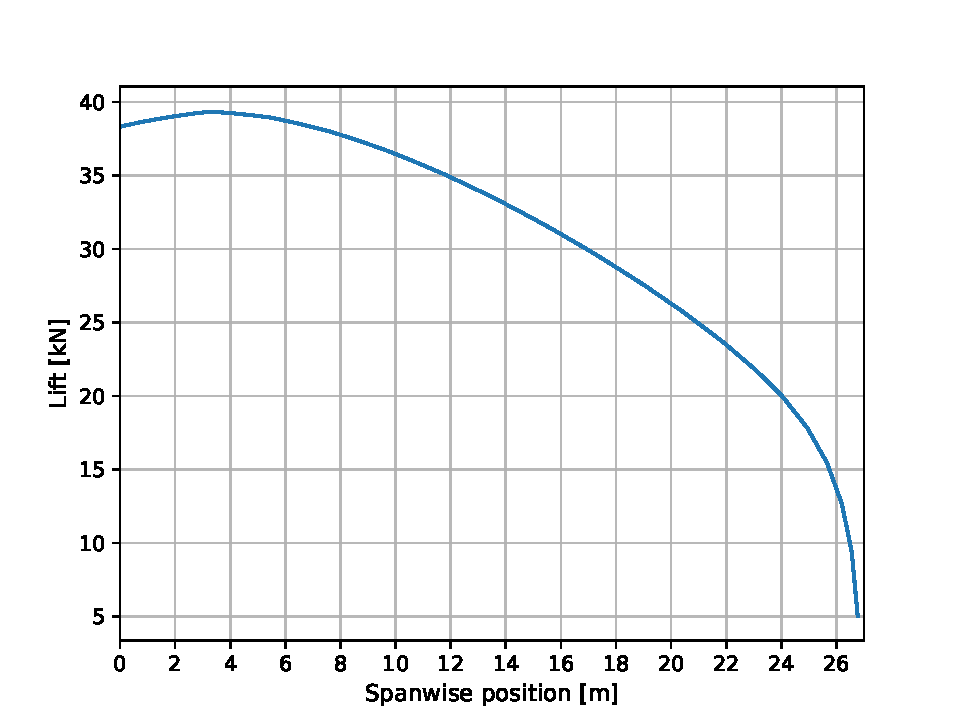
\includegraphics[width=0.7\linewidth]{figures/Lift distribution.pdf}
    \caption{Spanwise Lift Distribution}
    \label{fig:lift-distribution}
\end{figure}

\begin{equation}
    L=c_l q_\infty c \quad
    D=c_d q_\infty c \quad
    M=c_m q_\infty c^2
    \label{eq:Loads per unit span}
\end{equation}

\section{Shear Force, Bending Moment, and Torque}   \label{sec:fd_shear_moment_torque}
%Derivation of the shear force, bending moment and torque diagrams, and the corresponding plots. 

%Include two graphs for each plot: one corresponding to a critical load case with a positive load factor found in WP4.3, and one corresponding to a critical load case with a negative load factor found in WP4.3. Note that the inertial force on all elements depends on the load factor.
This section focuses on the formulae derivation and graphical representation of the shear force, bending moment, and torque acting on the wingbox. These are determined by the distributed aerodynamic loading, previously obtained in \autoref{sec:fd_aerodynamic_loading_analysis}. Specific numerical values and plots were obtained using a Python tool, the code for which can be found in \autoref{}\todo{ref Python appendix}.

\subsection*{Shear Force}
\noindent The shear force can be expressed in terms of the distributed wing loading as shown in \autoref{eq:shear_force_relation} \cite[p. 28]{Timmer2024AE2111-IReader}.

\begin{equation} \label{eq:shear_force_relation}
    w(x) = -\frac{dV}{dx}
\end{equation}
\noindent This expression can be integrated to obtain an expression for the shear force distribution along the wing as shown in \autoref{shear_force_integral}.
\begin{equation} \label{shear_force_integral}
    V(x) = \int^{b/2}_x{w(x)dx} - P(x)
\end{equation}
where $P(x)$ represents the shear force due to the weight of the engine.\\
The derived formula was subsequently implemented into the Python numerical tool (see: \autoref{})\todo{ref Python appendix}. The code is comprised primarily of a \textit{for} loop, which runs along the length of the wing and calculates the shear force at each point by integrating the normal force acting from the given point to the tip of the wing. Additionally, to account for the shear force caused by the weight of the engine, an \textit{if} statement is included to ensure that all shear values between the engine and the root of the wing will take the effect of the engine into account.\\

\noindent To simulate the critical load cases (explained in \autoref{sec:fd_critical_cases}, a load factor was incorporated into the calculations, which allowed for the proper scaling of the internal shear force. The results of the iterated numerical evaluations were plotted in the corresponding spanwise location. The resulting shear force distribution diagram is showcased in \autoref{fig:shear_force_load_cases}.

\begin{figure}[H]
    \centering
    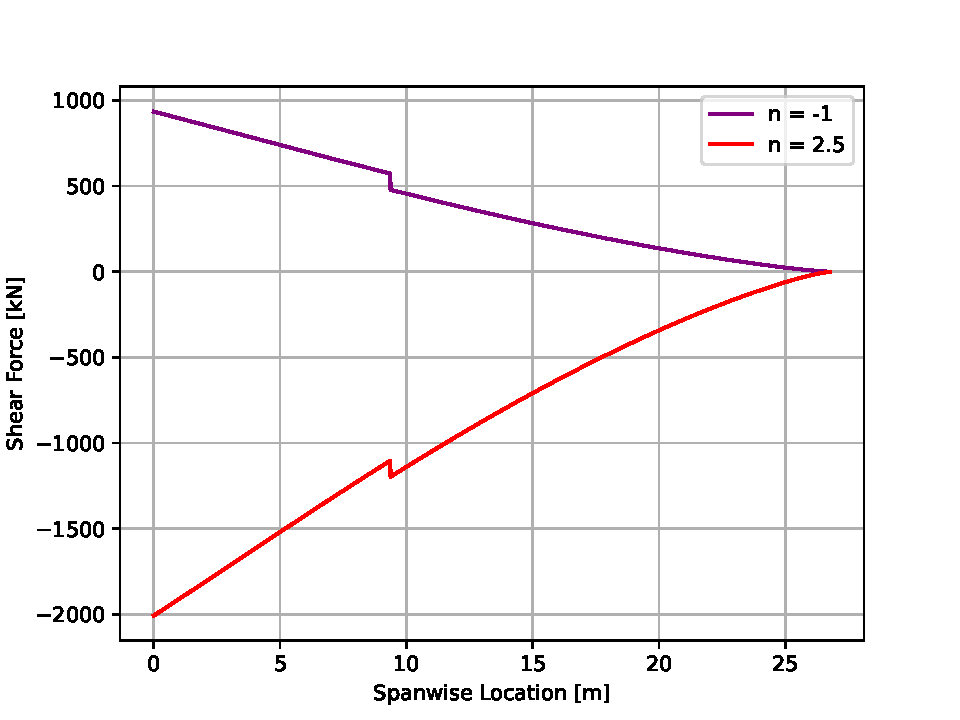
\includegraphics[width=0.8\linewidth]{figures/Shear_Force.pdf}
    \caption{Shear force distribution of critical load cases (load factor $n$ of $-1$ and $+2.5$)}
    \label{fig:shear_force_load_cases}
\end{figure}

\subsection*{Bending Moment}
The bending moment $M$ is generally expressed as the second integral of the distributed load function, and hence closely related to the shear force $V$. It can be calculated by integrating \autoref{eq:fd:moment_shear_relation} \cite[p.28]{Timmer2024AE2111-IReader} along the \textit{x}-axis.
\begin{equation}    \label{eq:fd:moment_shear_relation}
    V(x)=\frac{dM}{dx}
\end{equation}

\begin{comment}
Suppose a couple moment $M$ is applied at a location $x_2$ \todo{Would do nicely with a figure}. The bending moment at a given spanwise location $x$ can be expressed using \autoref{eq:fd_moment_at_x} \cite{Timmer2024AE2111-IReader}.
\begin{equation}    \label{eq:fd_moment_at_x}
   -M(x)=\int^L_x{V(x)dx}\space+M\left(1-u_{x_2}(x)\right)
\end{equation}
\noindent In this case, $u_{x_2}$ is the step function which attains a value of $0$ for $x<x_2$ and $1$ for $x\geq x_2$. In the case of an aircraft wing, a point moment would be a simplified representation of the bending relief provided by the engine weight $M_E$. The moment itself can be calculated as a product of the engine's weight $P_E$ and spanwise position $x_E$, i.e.:
\begin{equation*}
    M_E=P_E\cdot x_E
\end{equation*}

With $P_E$ and $x_E$ attaining the values of $(9630\cdot9.81)$ N and $9.37$ m, respectively, based on the results of propulsion system sizing from \textit{Further Aircraft Design} \cite{} \todo{cite WP3}. Substituting these values yields an engine bending relief moment $M_E$ of $885.187$ kNm.\\
\end{comment}
\noindent Since only the bending contributions of lift and engine weight are considered to act on the wing, and no additional bending moments are present in the load model, the internal bending moment $M$ at a given spanwise location $x$ can simply be evaluated as:
\begin{equation*}
    M(x)=-\int^{b/2}_x V(x)dx.
\end{equation*}



\subsection*{Torque}
% You may assume the shear center to coincide with the centroid of the wingbox cross-section
The torque acting on the wingbox is dependent on several factors and design parameters of the wing structure. One of these characteristics includes the location of the shear center (SC) of the wingbox. For now, it is assumed that the SC coincides with the centroid of the wingbox \cite{Timmer2024AE2111-IReader} - a location which at this design stage is still unknown.\\

\noindent The driving loads determining the torque distribution of an aircraft wing are the distributed lift, the weight of the engine, and the thrust force, the latter of which is pointed inward towards the fuselage at an angle equal to the wing half-chord sweep angle $\Lambda$, as explained in \autoref{sec:fd_modeling_approach_and_assumptions} (see: \autoref{fig:fd_assumptions_equivalent_unswept_wing}). Due to this shift, not all of the thrust will induce torque. This analysis will focus on the component perpendicular to the flexural axis, which is obtained by applying \autoref{eq:thrust_perpendicular}:

\begin{equation}
    \label{eq:thrust_perpendicular}
    T_{\perp} = T\cos(\Lambda)
\end{equation}

\noindent  with the half-chord sweep angle $\Lambda$ and is equal to $26.55$ deg. For a single-engine thrust of $467.1$ kN, this results in a perpendicular thrust force of approximately $417.8$ kN.\\

\noindent The distributed aerodynamic loading of the wing is assumed to be acting on the quarter-chord line of the unswept wing, which results in a moment arm $d(x)$ equal to a quarter of the chord at each spanwise position. The contribution of the weight of the engine to the internal torque distribution is calculated using the assumption of a point force acting at a distance of $3.5$ m from the leading edge of the wing. Since the centroid location is not known yet, it is temporarily assumed to coincide with the half-chord line. This means that the distance $d_2$ is equal to the half-chord length at position $x_E$ plus $3.5$ m. For the contribution of the thrust of the engine at position $x_E$, it is assumed that the point force acts at a vertical distance of one radius of the engine from the shear center, which translates to $d_1 = 2.085$ m for the designed case. \\

\noindent The engines are placed at $x_E = 9.37$ m from the center of the fuselage. The engine mass is equal to $9,630$ kg and the thrust of the engine is $467,060$ N.


\noindent The last element necessary to derive the torque distribution is the quarter-chord pitching moment $t(x)$. Combining all the discussed factors allows for the derivation of the torsion $\tau$ at a location $x$ along the wing span, according to \autoref{eq:torsional_distribution} \cite[p. 29]{Timmer2024AE2111-IReader}: 
\begin{equation}
    \tau(x) = \int_0^{x}[w(x)d(x) + t(x)]dx + T_{\perp}d_1 \left(1 - u_{x_E}(x) \right) - W_Ed_2\left(1 - u_{x_E}(x) \right)
    \label{eq:torsional_distribution}
\end{equation}
In which $w(x)$ is the distributed spanwise loading, $d(x)$ - the distance between the point of application of the distributed load and the shear center, $d_1$ - the vertical distance between the orthogonal component of the thrust force $T_\perp$ (applied at $x_E$) and the flexural axis. Moreover, $d_2$ is the distance between the application of the engine weight $W_E$ and the flexural axis.\\

\noindent To describe the effect the engine positioning has on the wingbox torque, Heaviside step functions are included in \autoref{eq:torsional_distribution} - $u_{x_E}$ attains a value of 0 for $x<x_E$ and the value of 1 for $x\geq x_E$. A visualization of the wing loading considered for torsion is shown in \autoref{fig:fd_torque_visualisation}.\\
\begin{figure}[H]
    \centering
    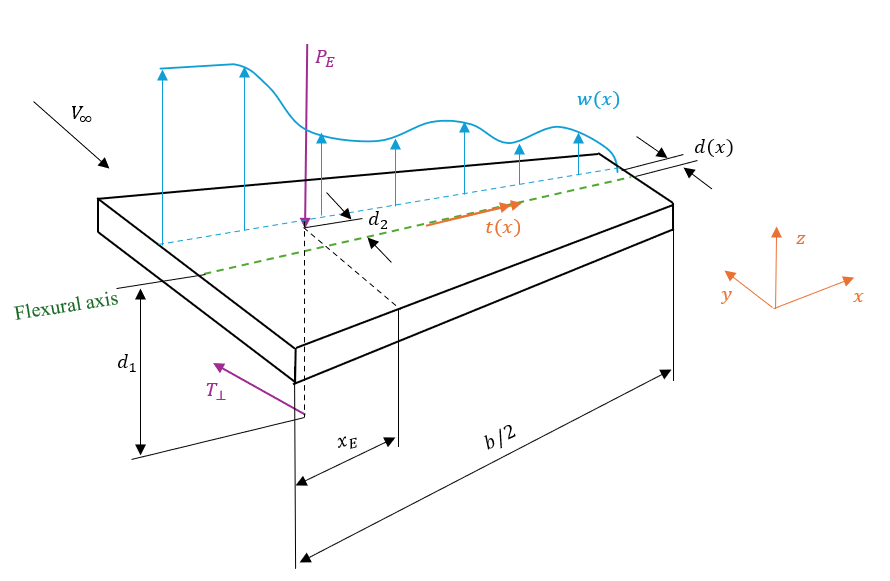
\includegraphics[width=0.8\linewidth]{figures/beam_loading_torsion.png}
    \caption{Visualisation of Wing Torque Derivation}
    \label{fig:fd_torque_visualisation}
\end{figure}

\noindent The internal torque of the wing is acquired by converting \autoref{eq:torsional_distribution} to a Python code. In this code, the quad function of the scipy library is used for the integration of the pitching moment and the distributed normal load times its moment arm. A for-loop is used to iterate over each spanwise position with steps of $0.01$ m to calculate the internal torque at that location. For the critical load cases with loading factors of $n = 2.5$ and $n = -1$, the torsional distribution is plotted in \autoref{fig:torque_diagram_load_cases}.

\begin{figure}[H]
    \centering
    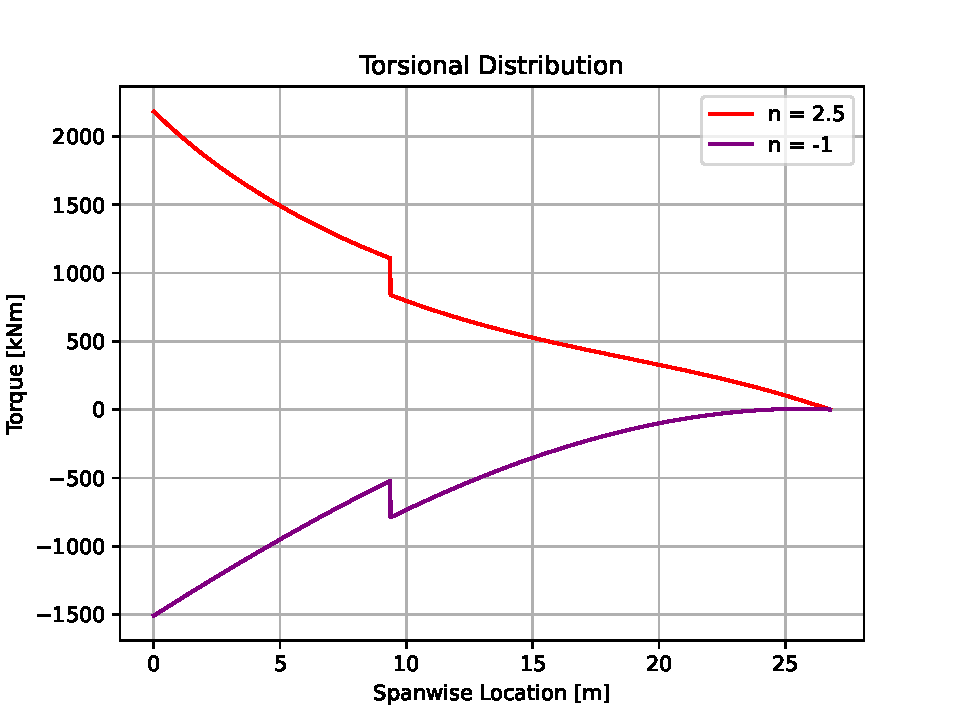
\includegraphics[width=0.8\linewidth]{figures/Torsional distribution of critical load cases.pdf}
    \caption{Torsional Distribution for Critical Load Cases}
    \label{fig:torque_diagram_load_cases}
\end{figure}

\section{Explanation of Critical Cases} \label{sec:fd_critical_cases}
% Justification on why these load cases can be considered as the most critical
In Sections \ref{sec:fd_modeling_approach_and_assumptions}-\ref{sec:fd_shear_moment_torque}, a numerical tool was developed to calculate and plot the distributed loads acting on the wing. Its purpose was to analyze the impact of flight conditions on the wing structure. In \autoref{ch:Prelim_WB_Des}, loading cases are considered for a set of conditions. Based on this, two \textit{critical load cases} were defined: one for a positive load factor $n$ of $+2.5$ at dive speed $V_d$, and one for a negative value of $-1$ at cruise speed $V_c$. Both of these load cases corresponded to an aircraft at its maximum payload weight (MPW), with fuel weight included. The details of both cases are shown in \autoref{tab:fd_crit_loadcases}.


\begin{longtable}{|>{\columncolor{blue!15}}c|p{3.2cm}|p{2cm}|c|c|c|p{2.6cm}|}
\caption{Table of considered Load Cases}
\label{tab:fd_crit_loadcases}
\endfirsthead
    \hline
    \rowcolor{blue!15} \textbf{Load Case} & \textbf{Description} & \textbf{Speed$_{EAS}$ [m s$^-1$]} & \textbf{Altitude} & \textbf{Weight [kN]} & \textbf{n} & \textbf{Comments} \\
    \hline
    LC-21 & $OEW+MPW+\text{fuel}$, sea-level at $V_{d}$ & 362.94 & FL0 & 1803.4 & 2.5 & Trimmed HLDs (clean config.) \\
    \hline
    LC-22 & $OEW+MPW+\text{fuel}$ at $V_{d}$, sea-level at $V_{c}$ & 241.96 & FL0 & 1803.4 & -1 & Trimmed HLDs (clean config.) \\ 
    \hline
\end{longtable}
The critical cases for shear can be observed by plotting the shear distribution for every load case and then selecting only the distributions which are on the boundary of the plot. As it can be observed, for shear, only the LC-21, LC-22 and LC-27 represent the critical cases. \todo{(note for feedback) graphs for torsion and moment are still in progress, but the same principle will be applied for them too as for the shear }
\begin{figure}[H]
    \centering
    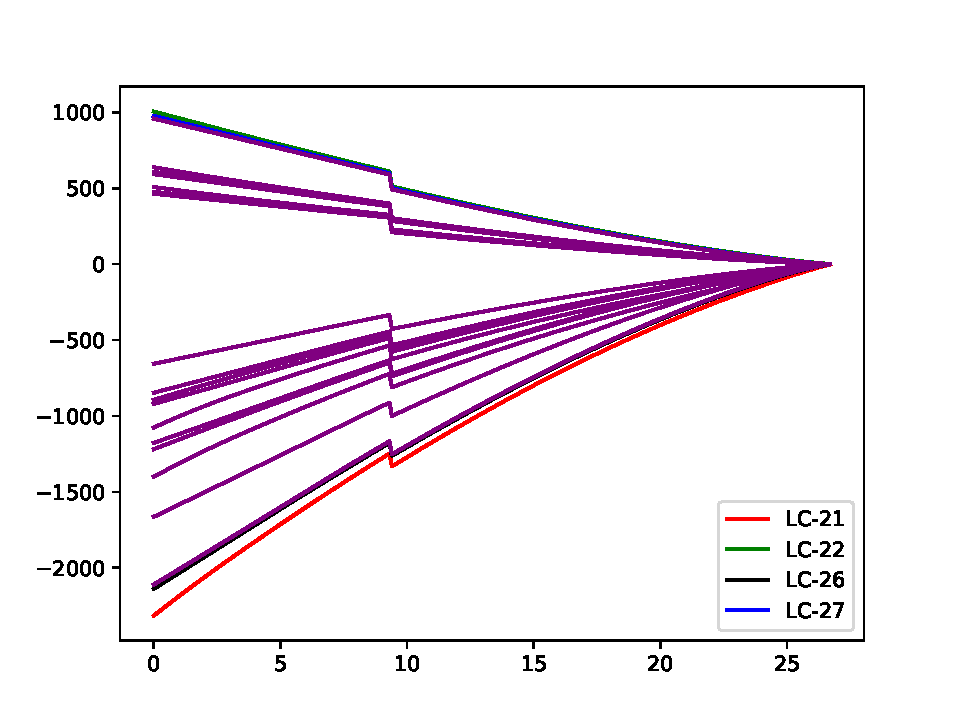
\includegraphics[width=1\linewidth]{figures/Shear load case.pdf}
    \caption{Shear distribution for all the load cases}
    \label{fig:enter-label}
\end{figure}